%Set up the document and load packages
\documentclass[letterpaper, 12pt]{article}

%---------------------------------------- + ---- + ---- + ---- + 
\setlength{\parskip}{1ex plus0.5ex minus0.5ex}
\setlength{\textheight}{9.0in}
\setlength{\textwidth}{6.5in}
\setlength{\topmargin}{-0.5in} %% remove if using latex, rather than pdflatex
\setlength{\oddsidemargin}{0in}
%---------------------------------------- + ---- + ---- + ---- + 
\usepackage[T1]{fontenc}
\usepackage[utf8]{inputenc}
\usepackage{amsmath}
\usepackage{lmodern}
\usepackage{adjustbox}
\usepackage{blindtext}
\usepackage{isotope} %Makes it easier to write isotope superscripts
\usepackage[table]{xcolor}% http://ctan.org/pkg/xcolor
\usepackage{array} 
\usepackage{siunitx} %SI units
\usepackage[width=.75\textwidth]{caption}
\usepackage[english]{babel}
\usepackage[autostyle]{csquotes}
\usepackage{pdfpages}
\usepackage{textcomp} %for trademark and copyright symbols
\usepackage{graphicx} %for adding figures
\usepackage{natbib} %to get author-year citations
\bibpunct{(}{)}{,}{}{}{,} %defines how citation punctuation works
\usepackage{lineno} % for line numbering
\usepackage{setspace} %\doublespacing
\usepackage{rotating}
\usepackage{float} %to get displays to stay where one puts them
\usepackage{hyperref} %use this to add URLs conveniently

%%%%%%%%%%%%%%%%%%%%%%
% Begin the document %
%%%%%%%%%%%%%%%%%%%%%%

\begin{document}

\noindent {\large \bf The title of your amazing work!} 

\medskip

\noindent {\large Your name\textsuperscript{1}}

\bigskip   

\noindent \parbox[t]{6.5in}{\textsuperscript{1}Department of Botany, University of
  Wyoming, Laramie, WY 82071, USA}

\vspace{2in}

\noindent \emph{Corresponding author}: \parbox[t]{4in}{Your Name\\
  1000 E. University Ave.\\
  Department of Botany, 3165\\
  University of Wyoming\\
  Laramie, WY 82071, USA\\
  youremail@uwyo.edu\\
  Fax: who still uses this?
}

\bigskip

\noindent 
\emph{Keywords:} stuff, major good stuff, really good stuff, crap

\bigskip
\noindent \emph{Running title: Reproducibility!}

\bigskip

\noindent Author contributions: XYZ
\newpage

%%%%%%%%%%%%%%%%%%%%
% Begin manuscript %
%%%%%%%%%%%%%%%%%%%%

\section*{Abstract}
How to use Make, Git, R, and \LaTeX to do great things (more than once).



\begin{linenumbers} %Turn on line numbering.
\section{Introduction}
We will do XYZ because of XYZ. 

A benefit of \LaTeX is citation incorporation. You can source a bib file and make use of any of the citations therein with the citep, citet, citalt, and other cite commands. For more see: \href{https://www.imperial.ac.uk/media/imperial-college/administration-and-support-services/library/public/LaTeX-and-BibTeX-branded-jan-2016.pdf}{Citing tutorial}

Look into the variations of the "cite" command for extra functionality. 

RECOMMENDED: You can also link your citation manager to your overleaf project. See how to do that here: \href{https://www.overleaf.com/learn/latex/Bibliography_management_with_bibtex}{Using a citation manager}

This is very handy since you can simply refresh as needed to quickly bring new citations into your manuscript. Note where we define the bibliography after the acknowledgements. At that point we specify style. You can download citation styles for many journals, so never reformat citations by hand!

\section{Methods}
Check it out, we did XYZ

\section{Results}
Here are the results from X (Fig.~\ref{fig:scatterplot}). Note that the number of the figure is automatically updated based on its order in the figure section.

\section{Discussion}

\section*{Acknowledgments}
Funding was provided by XXXX. Computing was performed in the Teton Computing Environment at the Advanced Research Computing Center, University of Wyoming, Laramie (https://doi.org/10.15786/M2FY47).

\section*{Data availability}
All scripts and processed data are available at:
https://bitbucket.org/harrisonjg/asle\_microbiome\_manipulation/src/master/ 

\end{linenumbers}

%%%%%%%%%%%%%%%%%%%%%
% Make bibliography %
%%%%%%%%%%%%%%%%%%%%%

\bibliographystyle{apa}
\bibliography{Zotero.bib} %Zotero is free and works great

%%%%%%%%%%%%%%%%%%%%%%
% Figures and tables %
%%%%%%%%%%%%%%%%%%%%%%


\pagebreak
\begin{figure}[H]
    \centering
    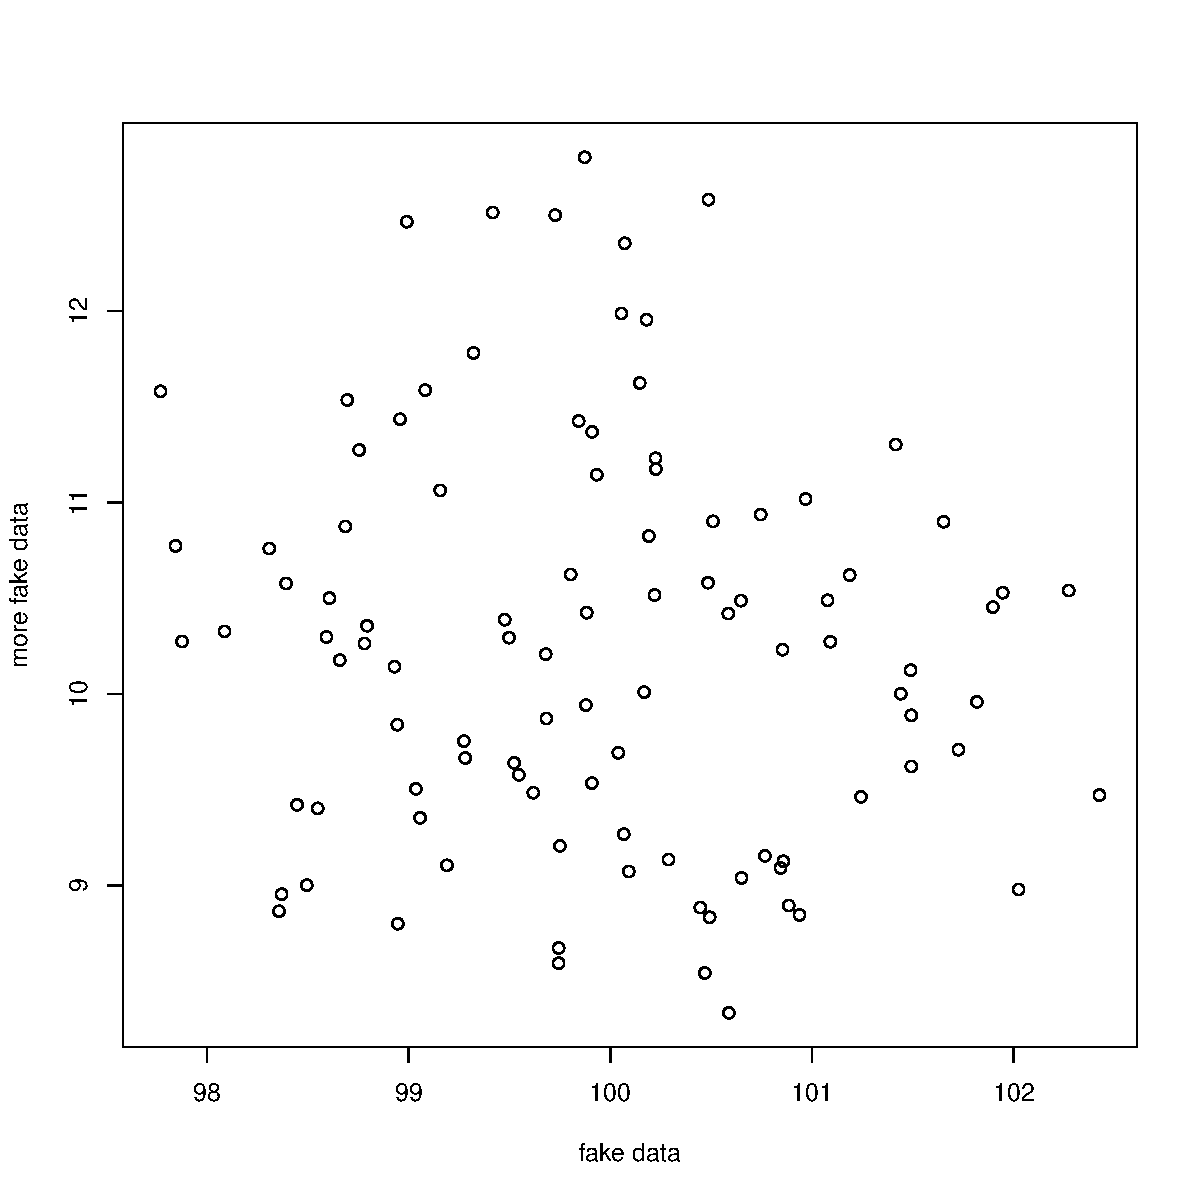
\includegraphics[width=0.9\linewidth]{./results/scatterplot.pdf}
  \captionsetup{width=0.75\textwidth}
  \caption{A scatterplot of some random data}
    	\label{fig:scatterplot} %Use this label to reference the figure in the text.
\end{figure}

%Example code to render a table
\pagebreak
\begin{table}[H]
    \centering
	\caption{Example Simple table.}
	\label{table:simpleExample}
	\begin{tabular}{ccc} %lrc means left, right, or center justified
    \hline
	Treatement 1 & Treatment 2 & Sample size \\
    \hline
	 Yes & Yes & 62\\
	 Yes & No & 68\\
	 No & Yes & 54\\
	 No & No & 54\\
	 \hline
    & Controls & \\
    \hline
     Yes & Yes & 13\\
	 Yes & No & 13\\
	 No & Yes & 18\\
	 No & No & 18\\
	\hline
	\end{tabular}
\end{table}

%Or, we can source tables output directly from R, a way better solution!
% latex table generated in R 3.4.3 by xtable 1.8-3 package
% Fri Mar  1 12:22:13 2019
\begin{table}[ht]
\centering
\caption{Results from a regression of a simulated vector of deviates from a normal distribution centered at 100 against deviates from a normal distribution centered at 10. xtable is awesome!} 
\label{table:lm_results}
\begin{tabular}{cccc}
  \hline
Estimate & Std. Error & t value & Pr($>$$|$t$|$) \\ 
  \hline
101.24 & 1.06 & 95.10 & 0.00 \\ 
  -0.13 & 0.10 & -1.24 & 0.22 \\ 
   \hline
\end{tabular}
\end{table}


%%%%%%%%%%%%%%%%%%%%%%%%%
% Supplemental material %
%%%%%%%%%%%%%%%%%%%%%%%%%

\pagebreak
\subsection*{Supplementary Material}
%%% the following command will set up separate numbering for
%%% Supplemental Tables and Figures
\setcounter{table}{0} \renewcommand{\thetable}{S\arabic{table}}
\setcounter{figure}{0} \renewcommand{\thefigure}{S\arabic{figure}}

\end{document}
